\documentclass[12pt]{article}

\usepackage{hyperref} %links in ToC
\usepackage{caption} %interesting things with captions
\usepackage[margin=1.5in]{geometry} %mostly set margin of the report
\usepackage{tabulary} %text wrapping in tables
\usepackage{subcaption} %let me put multiple images into a single caption
\usepackage{textcomp} %let me use \textrangle{} to get '>'

%images being embeded
\usepackage{graphicx}
\graphicspath{ {images/} }

%code highlighting
\usepackage{minted}
\setminted[c++]{frame=single,linenos=true,autogobble=true,numbersep=4pt,tabsize=4}
\setminted[bash]{frame=single,linenos=true,autogobble=true,numbersep=4pt,tabsize=4}
\setminted[xml]{frame=single,linenos=true,autogobble=true,numbersep=4pt,tabsize=4}
\setminted[python]{frame=single,linenos=true,autogobble=true,numbersep=4pt,tabsize=4}

%fix a quote mark issue
\usepackage [english]{babel}
\usepackage [autostyle, english = american]{csquotes}
\MakeOuterQuote{"}


\begin{document}
\pagenumbering{gobble}
\begin{titlepage}
	\centering
	{\Huge C++ Threading\par}
	\vspace{0.25in}
	{\Large Project 1\par}
	\vspace{2in}
	{Alex Harper\par}
	\newpage
\end{titlepage}
\pagenumbering{roman}
\tableofcontents
\newpage

\listoffigures
% \listoftables
\newpage
\setlength{\parindent}{4em} %indent of first line of paragraph
\setlength{\parskip}{1em} %space between paragraphs

\pagenumbering{arabic}

\section{Introduction}

Many modern computers have multiple processors allowing for multiple instruction streams to run at the same time.
Even before having this hardware, operating systems had created mechanisms to run multiple process "at the same time" to solve some common problems.
Because of this transaparent ability of systems to run several things at once, it has become fairly common for programs to use multiple threads; each thread being responsible for different tasks.

C++ has traditionally relied on external frameworks or APIs to have this functionality.
This is because it stems from C which had the philosophy of being simple and generic in the early days fo computing.
It was made in the time of still developing "multi-user" operating systems, which was the first major push for having time-sharing between programs.
Even with all that time, it was only in 2011 that C++ decided to add into their standard some items for doing threading.

\section{Basics}

There are a few concepts that all threading systems have.
Even with different systems, the ideas you learn can typically be translated between them.
Since this is a simple report to show I know the material, I will keep things on a more overview level.

\subsection{Threads}

The first concept is that multiple things are going at the same time.
Looking at the psuedo code below, you can see how this can manifest.
Since we ask the computer to run two functions at the same time, they both step over each other trying to print.
That is why the output is a jumble between the two functions.

\begin{figure}[htb]
	\centering
	\begin{tabular}{l|l}
		\hline Code &
		\begin{minipage}[t]{0.4\textwidth}
		\begin{minted}[frame=none,linenos=false]{python}
			print_0_3():
				print 0
				print 1
				print 2
				print 3
			print_4_7():
				print 4
				print 5
				print 6
				print 7
			start_thread(print_0_3)
			start_thread(print_4_7)
		\end{minted}
		\end{minipage}
		\\ \hline
		Output &
		\begin{minipage}[t]{0.4\textwidth}
		\begin{verbatim}
			0 4 1 5 2 6 3 7
		\end{verbatim}
		\end{minipage}
		\\ \hline
	\end{tabular}
	\caption{Example of Mutiple Things Happening at Once}
\end{figure}

\newpage
Ah, but you can never expect it to work exactly like that every time.
Computers are stupidly complicated these days, and so even running the same code, you might get something like below.
Different things cause it to change; which core each thread is put on, when interupts happen, load on the computer, varying speed of the processors, etc.

\begin{figure}[htb]
	\centering
	% \begin{verbatim}
		0 1 4 2 3 5 6 7
	% \end{verbatim}
	\caption{Second Example Output}
\end{figure}

\subsection{Locks}

Since you can never be sure when things will happen, that can lead to some problems.
Lets stick to only two threads for an example.
1 decides to do some work popping an item off a stack, 2 waltzes in and decides to do the same.
1 is busy with changing the pointer on the stack and decrementing the count variable but gets told to pause.
2 now has a pointer that got changed, but the counter variable had not quite yet changed.
when 1 comes back after 2 does its thing, the pointer was changed a second time for 2, but 1 doesn't know that.
So it decides to write the size it remembered to the variable for how full the stack is.

This pause between parts of its work is what causes a lot of problems (and other more complicated stuff).
The stack is now saying it is x-1 large even though it had two items popped off of it, meaning the size it returns will be wrong from now on.
So how can you keep this from happening?
Obviously using the title of this section.

Locks are something that is guarenteed to be safe to be used across threads.
They are something you "lock" and then do your work.
With our two threads, 1 wants to do its work, so it "locks" the lock and then carries on like normal.
When it gets paused and 2 tries to do the work, it is transparently told to wait because the lock is already "locked".

Some simple example code below to show a semi-specific way of how it looks.
These locks are often in the form of a mutex.
A mutex allows only one process to hold the lock at a time, and all others will try and be told to pause until it is unlocked.

\begin{figure}[htb]
	\centering
	\begin{minipage}{0.4\textwidth}
	\begin{minted}{python}
		pop_stack():
			try_lock(mutex)
			stack.pop()
			unlock(mutex)
		start_thread(pop_stack)
		start_thread(pop_stack)
	\end{minted}
	\end{minipage}
	\caption{Example Mutexes}
\end{figure}

Locks are not always perfect, and they need discipline to be used correctly.
Lets keep with two threads, but this time we have two locks.
If thread 1 locks A then B, and thread 2 locks B then A at some point in the code, then there is a chance that 1 locks A, 2 locks B.
Then they are waiting on each other to realse the locks they dont have.

\subsection{Atomics}

"The Future Is Nuclear"  -- Silly Statement

Reguardless of how true the previous line is, multi-threading can make good use of atomics.
The root is atom, which means indivisible (unable to break up further).
Things that are atomic on the computer are things that are guarenteed to work safely across threads.
It is the equivilent of doing something instantly and so other threads can not interupt it.

Using locks like in the previous section, you can approximate this like adding locks to the stack internals so now the stack is thread safe.
But in many places, there is often a concept of marking variables as atomic.
This is often better to use than locks because there is often fast hardware support and you dont have to mess with a million different locks and assosiated problems.

When a variable is marked atomic, then you are free to assign and read it whenever you want, and other threads will not be able to interupt it.
Uses for it might be having a loop counter or a place you are adding up different results into.
This makes it safe for single lines of code to not have problems.

But only single lines.

\begin{figure}[htb]
	\centering
	\begin{tabular}{|l|l|}
		\hline
		Good & atomic\_int = 5; \\ \hline
		Good & atomic\_int += 3; \\ \hline
		Good & atomic\_int /= 2; \\ \hline
		Bad & atomic\_int = pow(atomic\_int,2); \\ \hline
	\end{tabular}
\end{figure}

Depending on language and framework constraints, it is often the case that the last line will not have proper guarentees.
The way it breaks is that the last line reads the variable (safe) and passes the value to pow() and then writes to it again (safe).
The problem is that the read and the write are seperate and so not under the same guarentees of each individual read and write.

\subsection{Efficency}

So now that the super basics are out of the way, lets talk about how well it will help your program run.

There is always overhead when using a lock or atomic since there is extra work to do.
This means that if you split a task up among multiple threads, it will be doing more work total, but also more work concurrently.
Ussualy it wins out having threads, but it might be slightly disapointing how much it improves.
The table below shows some example times for a hypothetical task.

\begin{figure} [ht]
	\centering
	\begin{tabular}{|l|r|}
		\hline
		& Time  \\ \hline
		1 thread&40 \\ \hline
		2 threads&25 \\ \hline
		4 threads&15 \\ \hline
		8 threads&17 \\ \hline
	\end{tabular}
	\caption{Hypothetical Task Time in Seconds}
	\label{sorting_time2}
\end{figure}

I am thinking about things on my little 4-core computer.
As you can see, the 2 threads does not cut the time in half due to overhead of some theoretical kind.
4 threads is similar, but the overhead is a little worse percentage wise.
This usually happens because you have more threads fighting for the same lock.
8 threads, that is actually worse than 4.
If the machine is only 4 cores, then it can only do 4 things at once, and so half the threads wont actualy be doing extra work.
The extras threads though still can contribute to overhead about grabing locks.

\newpage
\section{Good Old Fashioned Pthreads}

Since the early days of unix, simple APIs for doing things have been a staple.
Pthreads comes from this early time, and with their simple function calls allow programs to do multi-threading.
Many things have tried to make interfaces that were similar to what these have.

The way these work is simple for the most part.
There are c functions that you call and then the functions do the right things.
Since it is using the old C style, there are no objects but you keep an integer handle to know which thread you are talkig about.

\begin{figure}[htb]
	\centering
	\begin{minted}{c++}
		#include <pthread.h>
		//function we want different threads to run
		void* function_name(void* data);
		//a way to refer to out thread
		pthread_t handle;
		//get the thread running by telling it what function to run
		pthread_create(&handle,NULL,function_name,&pointer_to_data);
		//wait for the thread to finish
		pthread_join(&handle,NULL);
	\end{minted}
	\caption{Basic Thread Spawning}
\end{figure}

\begin{figure}[htb]
	\centering
	\begin{minted}{c++}
		//struct to hold the mutex we care about
		pthread_mutex_t handle;
		//get the lock ready to use
		pthread_mutex_init(&handle,NULL);
		{//Use the lock
			pthread_mutex_lock(&handle);
			something_important();
			pthread_mutex_unlock(&handle);
		}
		//after use, you need to destroy it
		pthread_mutex_destroy(&handle);
	\end{minted}
	\caption{Basic PThread Mutex}
\end{figure}

\newpage
\section{C++11 Standard}

They finally got around to deciding that it was good to have a vendor neutral API for threading.
This is a quick look at what the basics are for the new standard.
It feels like a nicer interface than what pthreads use, but you are at the mercy of compiler versions to have support.

\begin{figure}[htb]
	\centering
	\begin{minted}{c++}
		#include <thread>
		//function we want different threads to run
		void function_name(int parm1, char parm2);
		//get the thread running by telling it what function to run
		std::thread th(function_name,42,"X");
		//wait for the thread to finish
		th.join();
	\end{minted}
	\caption{Basic Thread Spawning}
\end{figure}

\begin{figure}[htb]
	\centering
	\begin{minted}{c++}
		#include <mutex>
		std::mutex m;
		{
			m.lock();
			something_important();
			m.unlock();
		}
		{
			std::lock_guard<std::mutex> guard(m);
			something_important();
			//implicitly gets unlocked
		}
	\end{minted}
	\caption{Basic C++11 Mutex}
\end{figure}

% \begin{figure}[ht]
% 	\centering
% 	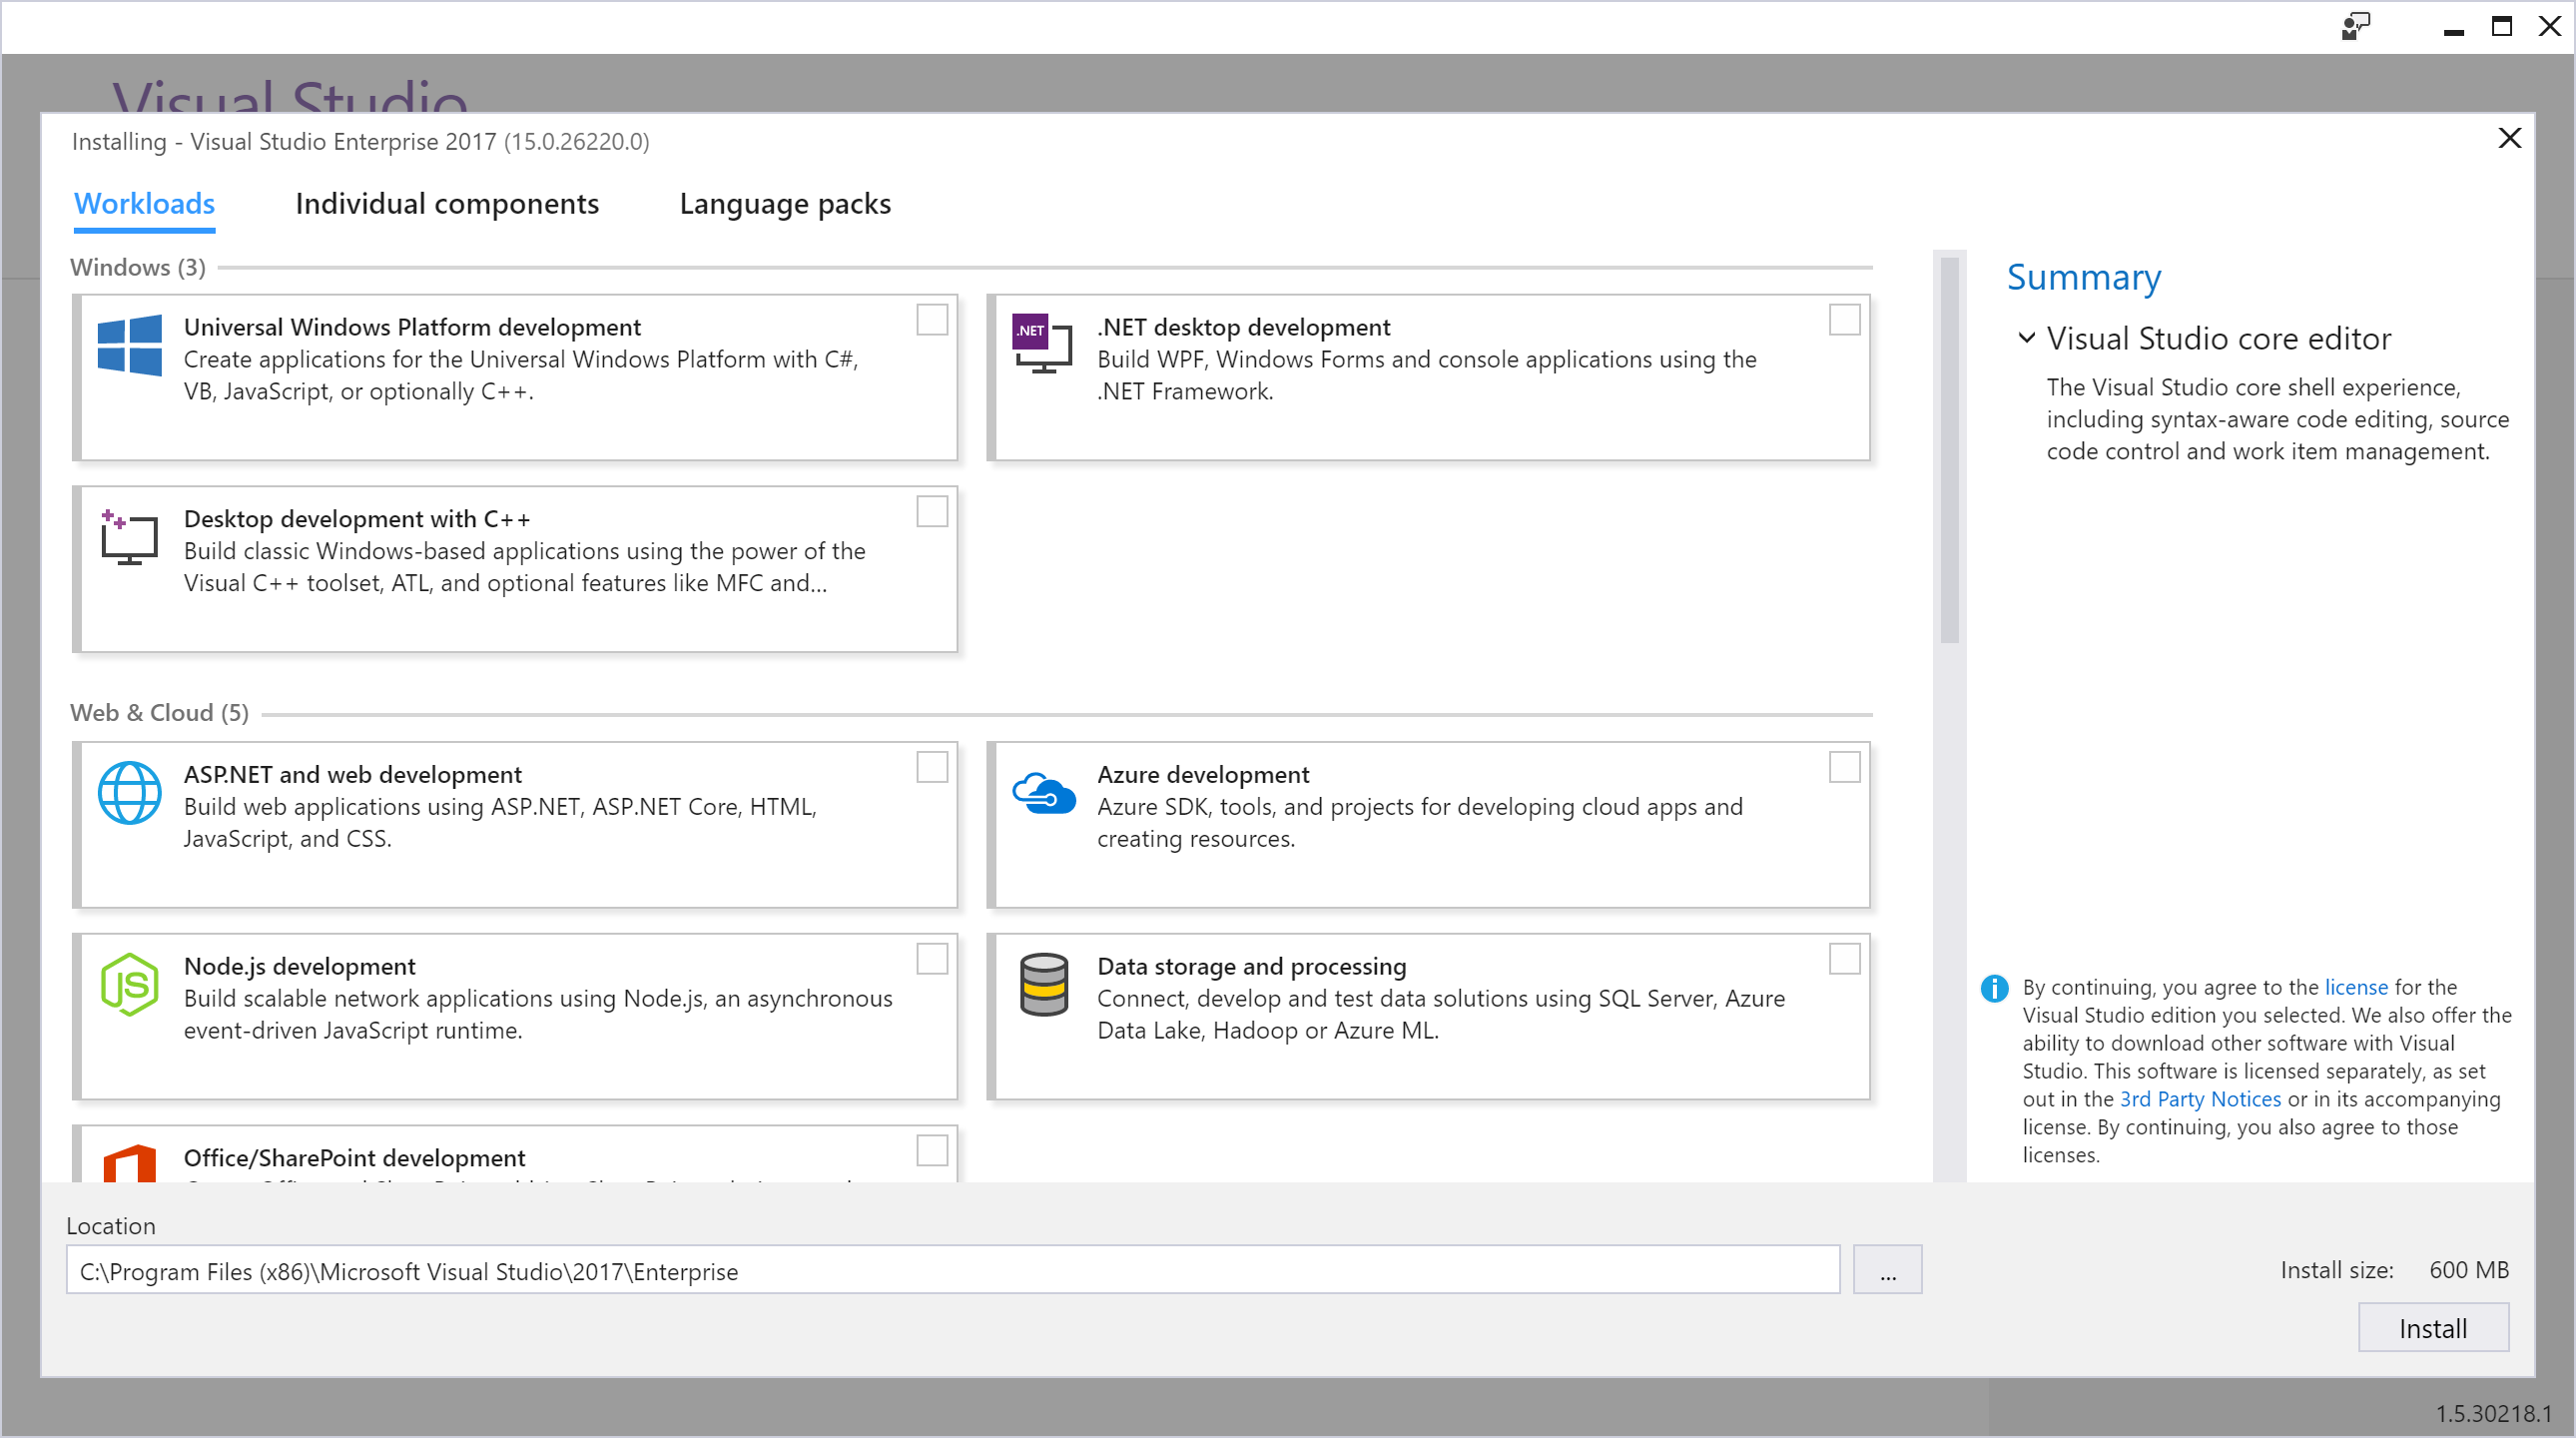
\includegraphics[width=\textwidth]{vs_installer.png}
% 	\caption{Window of Installer to Select extra Components}
% 	\label{fig:vs_installer}
% \end{figure}

\end{document}